%------------------------------------
% Document Preamble
%------------------------------------
\documentclass[12pt, a4paper]{article}
\setlength{\oddsidemargin}{0.5cm}
\setlength{\evensidemargin}{0.5cm}
\setlength{\topmargin}{-1.6cm}
\setlength{\leftmargin}{0.5cm}
\setlength{\rightmargin}{0.5cm}
\setlength{\textheight}{24.00cm} 
\setlength{\textwidth}{15.00cm}
\parindent 0pt
\parskip 5pt
\pagestyle{plain}

%------------------------------------
% Imported packages
%------------------------------------
\usepackage{graphicx}
\usepackage{lscape}
\usepackage{rotating}
\usepackage{siunitx}
\usepackage{wrapfig}

%------------------------------------
% Graphics path specification
%------------------------------------
\graphicspath{{./fig/}}

%------------------------------------
% Title block
%------------------------------------
\title{ENG720: Research Proposal}
\author{}
\date{}

\newcommand{\namelistlabel}[1]{\mbox{#1}\hfil}
\newenvironment{namelist}[1]{%1
\begin{list}{}
    {
        \let\makelabel\namelistlabel
        \settowidth{\labelwidth}{#1}
        \setlength{\leftmargin}{1.1\labelwidth}
    }
  }{%1
\end{list}}

\begin{document}
\maketitle

\begin{namelist}{xxxxxxxxxxxx}
\item[{\bf Title:}]
	To Be Confirmed
\item[{\bf Author:}]
	Shane Reynolds
\item[{\bf Supervisor:}]
	Charles Yeo
\item[{\bf Degree:}]
	Bachelor of Engineering (Honours)
\end{namelist}


%------------------------------------
% Contents
%------------------------------------
\tableofcontents
\newpage

%------------------------------------
% Introduction
%------------------------------------
\section{Introduction}

%------------------------------------
% Introduction
%------------------------------------
\section{Background}

\subsection{Power Systems and Frequency}
Interconnected power systems are comprised of power generating units and energy storage systems connected to transmission and distribution networks, where generated power is used to service load demand. A single line diagram of a power network can be seen in Figure 1. The left hand side of the diagram shows thermal generation units, such as coal and nuclear, in addition to renewable sources of generation, like wind and solar. The right hand side of the figure shows the distribution network and the consumers of generated energy: industry and households.
\begin{figure}[h]
	\centering
	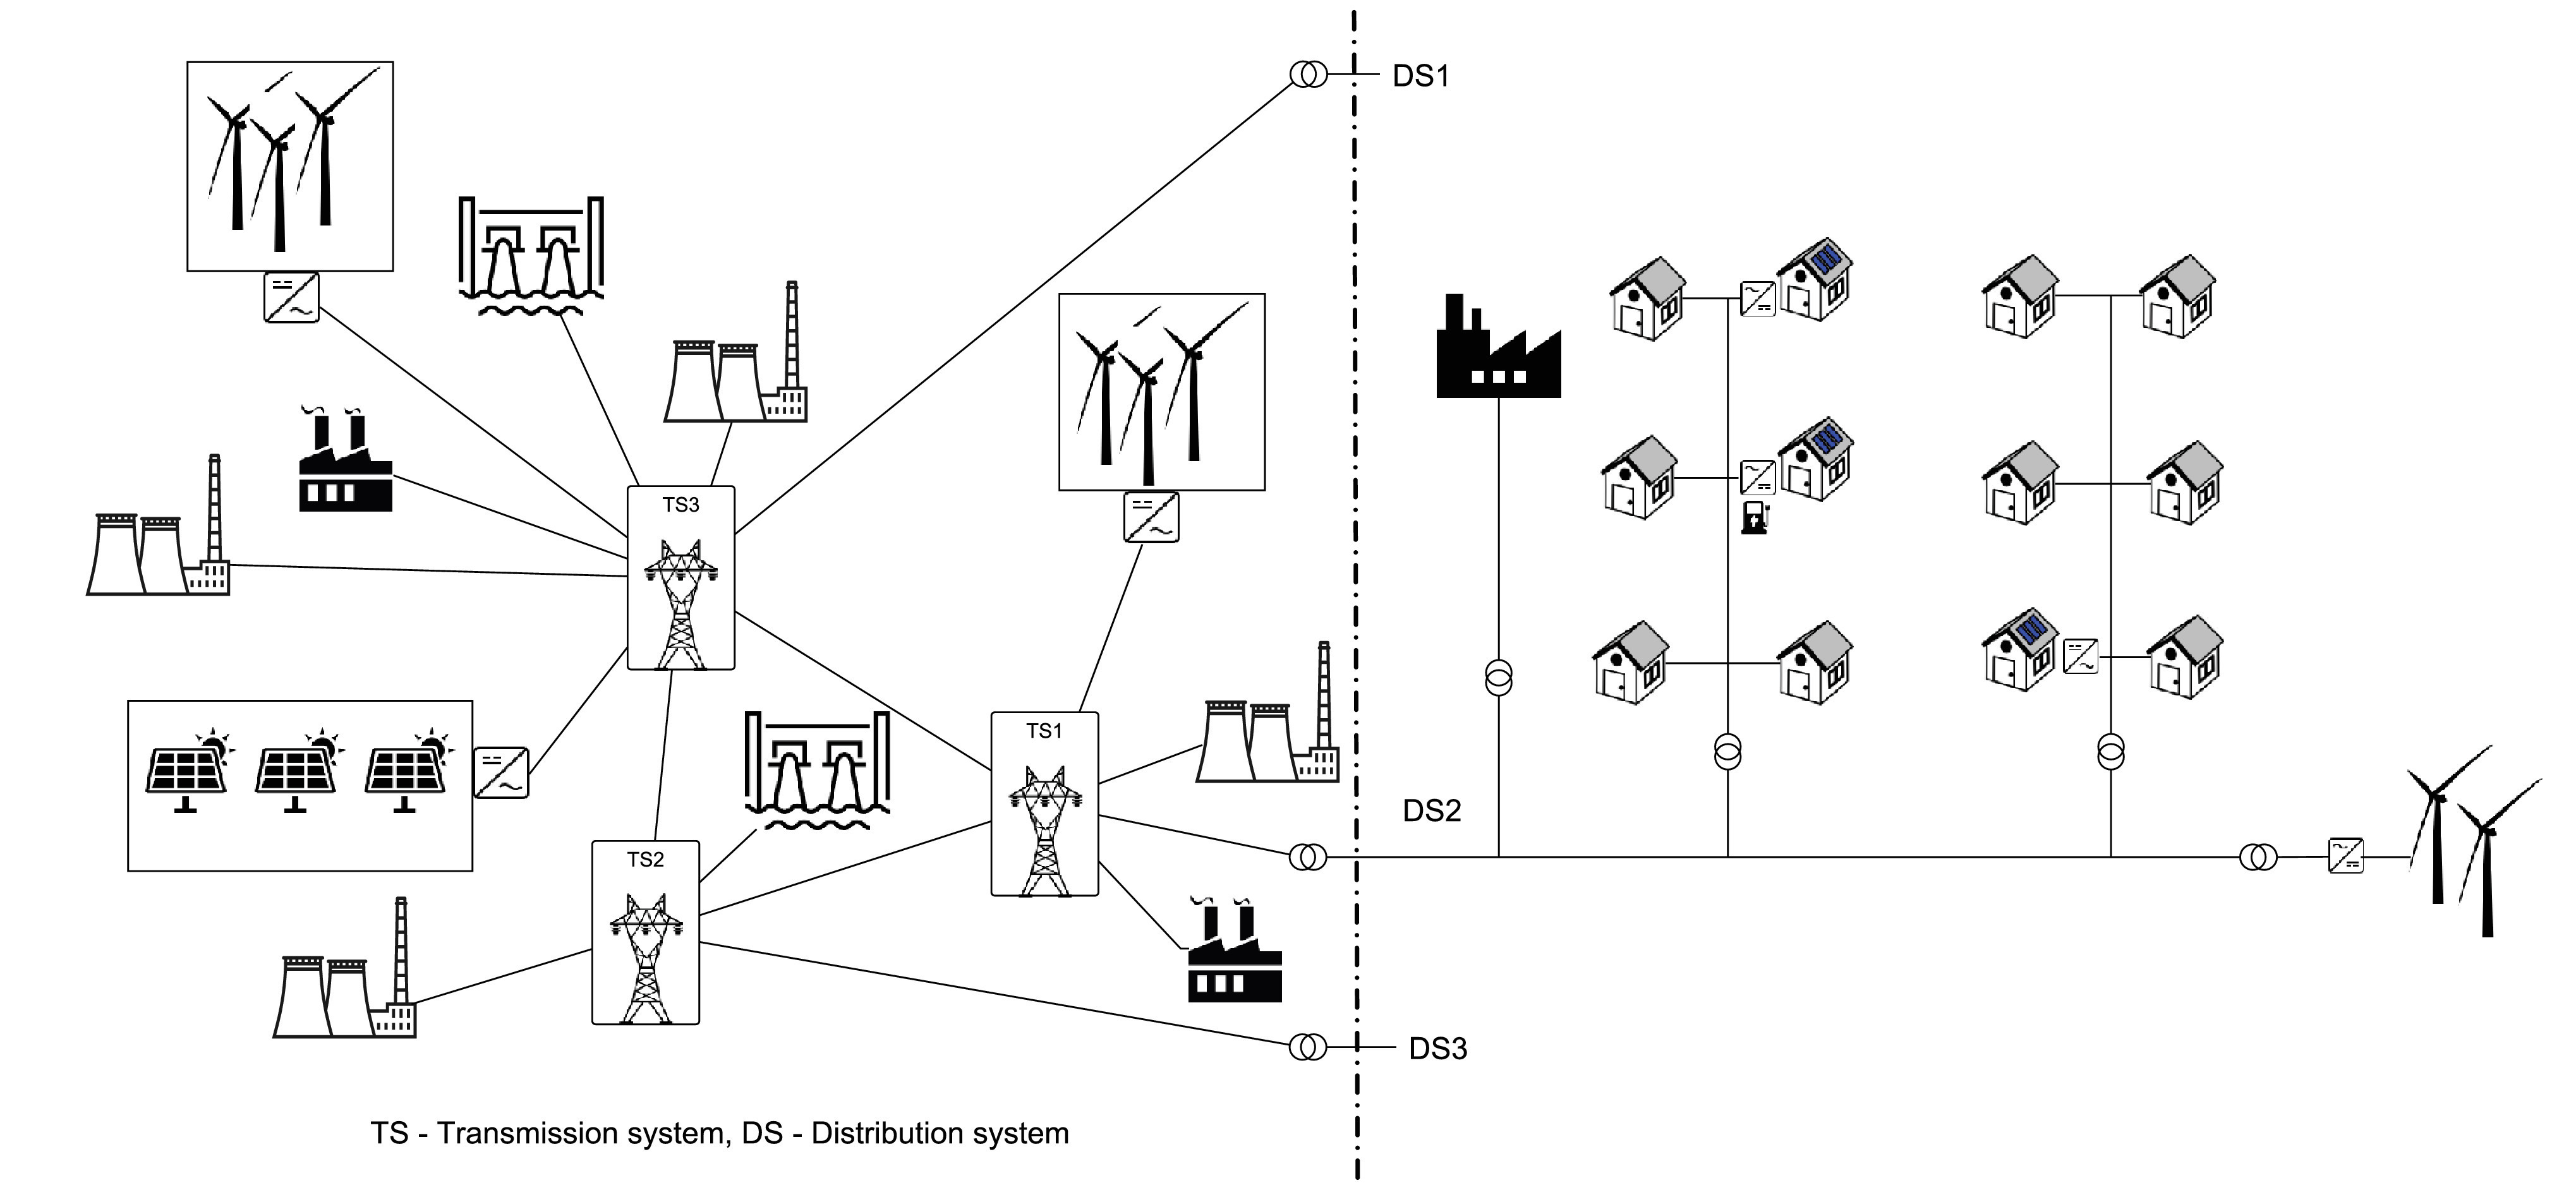
\includegraphics[scale=0.85]{power_system}
	\caption{A single line diagram of a typical power system taken from \cite{Glavic2019}. The image shows points of generation from thermal and renewable sources, and the subsequent supply of generated energy to meet load demand through the transmission and distribution network.}
\end{figure}

Successful operation of interconnected power systems requires total load demand to be matched with total generation, taking into account power losses involved with generation, transmission, and distribution \cite{Wood2013}. To understand why it is important to match generation with load demand it is useful to first consider the basic operation of a single thermal generator. The essential elements of a thermal generator are a prime mover (turbine) and a synchronous machine, as depicted in Figure 2.
\begin{figure}[h]
\centering
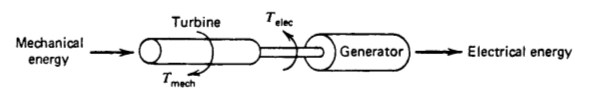
\includegraphics[height=1.4cm]{generation}
\caption{A thermal generation unit consists of a prime mover (turbine), and a synchronous machine. This image was taken from \cite{Wood2013}.}
\end{figure}

The prime mover provides mechanical torque, $T_{mech}$, which drives the synchronous machine producing electrical energy. In response, the synchronous machine creates a torque which opposes $T_{mech}$, dependent on the size of the load demand from households and industry. This is referred to as electrical torque and is denoted as $T_{elec}$. If $\alpha$ represents angular velocity of the generator rotating mass, and $I$ is the moment of inertia then by Newton's second law:
\begin{equation}
\sum T_i = I \alpha 
\end{equation}

Equation (1) shows that when $T_{mech}$ equals $T_{elec}$ the system will be in a steady state with zero angular acceleration, and a constant rotation at some angular velocity $\omega$. Now, if $T_{mech} > T_{elec}$, then the angular velocity $\omega$ of the system will increase as the system speeds up, resulting in a frequency increase in the system. Conversely, if $T_{mech} < T_{elec}$ then the angular velocity $\omega$ will decrease as the system slows down, resulting in a frequency decrease. What makes this situation interesting is that at any point in time the total electrical load demand will fluctuate stochastically, meaning that an uncontrolled system will have a continually changing frequency. System controllers, such as the Australian Energy Market Operator (AEMO) and Power and Water Corporation (PWC), can forecast daily demand profiles with some reliability using historical data. A plot of average historical data, for the daily demand profile in South Australia during Summer, can be seen in Figure 3.  
\begin{figure}[h]
	\centering
	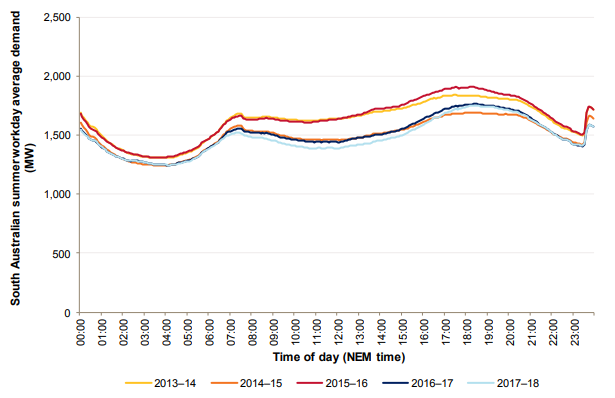
\includegraphics[height=7cm]{load_profile}
	\caption{Weekday energy demand profile in South Australia during summer \cite{AEMO2018}.}
\end{figure}

Forecasts provide a starting point that AEMO and PWC can use for estimating generation required to meet demand for some given time. Unfortunately, these forecasts are not perfect inevitably leading to mismatches in generation and load demand which cause small imbalances between $T_{mech}$ and $T_{elec}$, resulting in a change to angular velocity $\omega$ and the network frequency \cite{Glover2012}.\\ 

Australia's electricity network is designed to operate at a frequency of 50$\si{\hertz}$. In the majority of network scenarios AEMO has a desired operating range for frequency which lies between 49.85$\si{\hertz}$ and 50.15$\si{\hertz}$ \cite{AEMO2012}. Similarly, the PWC Network Technical Code for the Northern Territory states that under normal operating conditions frequency should be maintained in the range 49.80$\si{\hertz}$ to 50.20$\si{\hertz}$ \cite{PWC2018}. Operation outside of specified ranges can cause damage to electrical equipment (REFERENCE). Of course network designers engineer protection schemes so that sustained over or under frequency will generally cause equipment to trip from the network (REFERENCE). The same is true for large unexpected frequency deviations. Protection schemes tripping equipment from the network is undesirable since this can leave households and industry without power, resulting in economic loss. Further, if disconnections are uncontrolled then this can lead to a further loss of system stability (REFERENCE).\\

System controllers are therefore interested in being able to correct frequency deviations as quickly as possible. This is typically achieved using generators referred to as regulating units (REFERENCE). A regulating unit is a generator that has capacity to increase or decrease mechanical torque $T_{mech}$ allowing the system controller to arrest changing frequency and restore the system to stable operating conditions (REFERENCE). Often this capacity is referred to as a spinning reserve (REFERENCE). AEMO and PWC do not require all generators on the network to act as regulating units since adequate frequency control can be achieved using only a subset of the available generators (REFERENCE). A time series example of regulation action arresting a frequency disturbance, and the subsequent restoration of system frequency to normal levels, can be seen in Figure 4.
\begin{figure}[h]
\centering
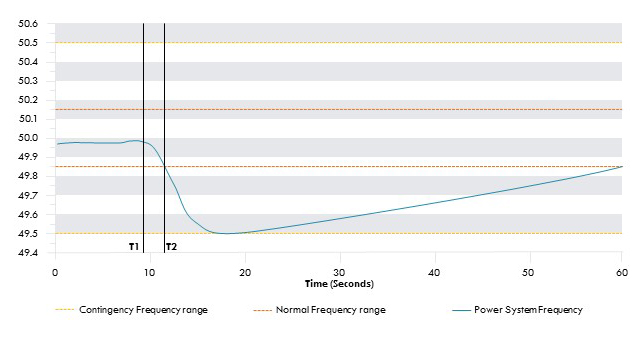
\includegraphics[height=8cm]{frequency_arrest}
\caption{A frequency disturbance occurs just before the 10 second mark, and regulating units ramp up their generation to first arrest the disturbance, and provide the subsequent correction, returning system frequency to 50$\si{\hertz}$.}
\end{figure}

Regulation needs to be performed quickly in response to a frequency disturbance. HOW QUICKLY DO UTILITIES NEED TO RESPOND. Typically regulation is performed automatically, except under highly abnormal operating conditions.

\subsection{Load frequency control for a single area}
The power system model shown in Figure 1 depicts total generation coming from many generation assets. Researchers often find it useful to divide generation assets into sub-groups referred to as control areas. Kothari defines a control area as a subset of generators belonging to a close knit area which constitute a coherent group such that all the generators speed up and slow down together maintaining their relative power angles \cite{Kothari2011}. The total network is therefore comprised of many interconnected control areas. An example of a series of interconnected control areas can be seen in Figure 5. Although there may be many generators and many loads present in a single control area, often researchers express these as a single generator, and single load, respectively \cite{Grainger1994}.
\begin{figure}[h]
	\centering
	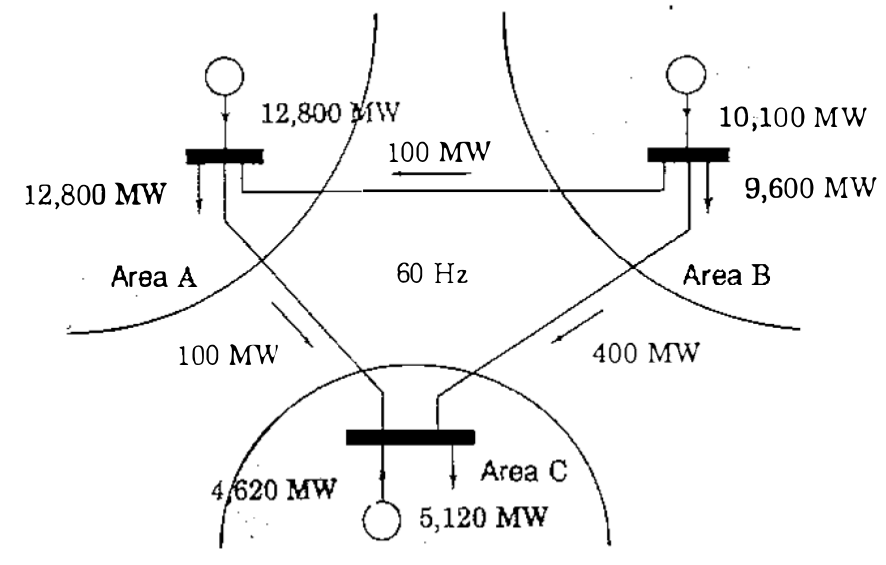
\includegraphics[height=8cm]{multiple_area_system}
	\caption{An example of three interconnected control areas in a 60$\si{\hertz}$ power system. The interconnections allow power to flow from one area to another, allowing generators to service loads from different areas. Each control area is consists of many generators and loads, but are modelled with a single generator and single load, respectively \cite{Grainger1994}.}
\end{figure}

The simplest power system to control is one that consists of a single control area, say Area A in Figure 5. This power system has no interconnections to any other network. It is comprised of consumer load demand, and a set of generators, some of which are acting as regulating units. For modelling simplicity, the loads are aggregated to a single load, and generators are aggregated to a single generator as with the multi-area system depicted in Figure 5. This classic, simple system is well understood and it is generally acknowledged that a governor feedback control regime can successfully perform frequency control of the system \cite{Wood2013, Grainger1994, Kothari2011}. Most introductory textbooks on power systems cover governor control of this system. Kothari provides a particularly well laid out approach to developing linear models for the turbine, generator load, and governor for the system. The full model can be seen in Figure 6 \cite{Kothari2011}. The first block is a first-order linear model of the speed governor, the second block is a first-order model of the turbine, which the controller directly acts on. The final block is the generator load, which is also a first order system. The over all system model is a second order linear model, with a first order controller.

\begin{figure}[h]
\centering
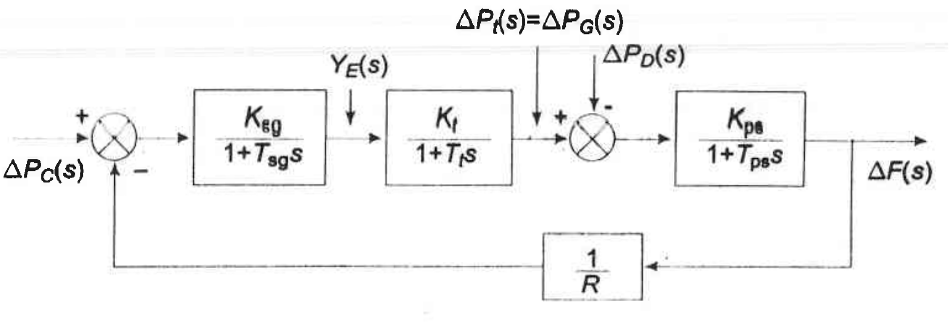
\includegraphics[height=5cm]{single_area_control}
\caption{A classical feed back control approach to a second order linear system. The second order system is comprised of a first order model for both the turbine, and generator load. The controller is modelled as a first order system \cite{Kothari2011}.}
\end{figure}


\subsection{Two-area load frequency control}
The system presented in Section 2.2 is useful to help understand the role of governors in controlling power system frequency, however, a single area model over simplifies things. In reality, power systems are comprised of many control areas connected through tie lines, which are typically transmission lines, though not always (REFERENCE). These distinct control areas are often thought of as different participants in the generation market, or simply as different regions in which generation assets are based (REFERENCE). To model the effects of tie lines, many researchers use a simple two area power system (REFERENCE). 

\begin{figure}[h]
	\centering
	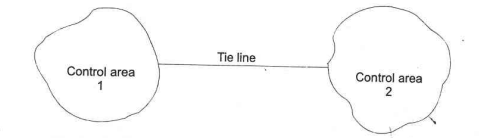
\includegraphics[height=3cm]{two_area_system}
	\caption{Two area power system is comprised of generators and load connected via a tie line. Power flows from one area to the other depending on economic contracts.}
\end{figure}

Two area power systems are well understood. Linear models have been developed, and classical control approaches analysed using governors on both

TALK ABOUT WHAT HAPPENS IF WE JUST LET THE SPEED GOVENORS DO THE JOB

TALK ABOUT HOW THIS MAY END UP VIOLATING ECONOMIC CONTRACTS THAT ARE IN PLACE

INTRODUCE AUTOMATIC GENERATION CONTROL AND THE ITS PRIMARY MOTIVATION

TALK ABOUT THIS LARGELY BEING A SOLVED PROBLEM

\subsection{Reinforcement learning}

TALK ABOUT THE HISTORY OF REINFORCEMENT LEARNING

TALK ABOUT APPLICATIONS IN THIS FIELD

\subsubsection{Markov Decision Process}
Reinforcement Learning (RL) is a branch of machine learning that is concerned with how agents make sequential decisions to maximise some notion of a cumulative reward. Suppose that a robotic agent exists in some environment which is comprised of many discrete states, $s \in S$, such that $S$ denotes the state space. At any discrete point in time the agent can take an action $a \in A$, where $A$ denotes the action space. When the agent takes an action in a given state, the agent receives some reward, denoted with $r \in R$, where $R$ is the reward set. If an agent is in a given state, $s$, and takes and action, $a$, this will transition the agent to a new state, $s'$, and yield reward, $r$, with some given probability - these are referred to as state transition probabilities. Transition probabilities are denoted as follows:
\begin{equation}
P(S_{t+1}=s', R_{t+1}=r \ | \ S_t = s, A_t = a)
\end{equation}

The set of parameters, outlined above, make up a framework referred to as a Markov Decision Process (MDP).

\subsubsection{Policy}
In order for the robot to act within the environment, it needs to have a policy. A policy, $\pi$, is defined as a mapping from states to actions, that is, a rule which determines what action the robot will take for a given state. A deterministic policy, $\pi (s)$, maps a single action to a single state. A stochastic policy, $\pi (a | s)$, defines a probability distribution over the actions for a given state.

\subsubsection{Return}
As the robotic agent takes actions at each discrete time step, it receives a reward. The cumulative sum of this reward is referred to as the return. The return is denoted, for $N$ discrete time steps, as:
\begin{equation}
G_t = r_t + r_{1+1} + r_{t+2} + \ldots + r_{N-1}
\end{equation}

Often it is convenient to make future rewards less important that more immediate rewards. This is by multiplying each reward in the sequence by a discount factor, $\gamma \in [0,1]$. Equation (XXXX) then becomes:
\begin{equation}
G_t = r_t + \gamma r_{1+1} + \gamma^2 r_{t+2} + \ldots + \gamma^{N-1} r_{N-1} = \sum_{k = 0}^{N-1} \gamma^k r_{t+k}
\end{equation}



TALK ABOUT THE BASIC COMPONENTS OF HOW IT IS PUT TOGETHER



\subsection{Deep reinforcement learning}

TALK ABOUT HOW DRL DIFFERS TO STANDARD RL

For low dimensional problems MC methods or TD methods see reasonable performance, however, as problem dimensionality of grows these approaches experience difficulty. The main reason for this is simply that it becomes difficult for the discrete RL algorithm to visit every state action resulting in unchanged \textit{state-action} values for an increasing number of \textit{state-action} pairs. Essentially this means that the agent does not have complete knowledge of optimal actions for every given state, leading to the derivation of sub-optimal policies. To get around this problem, for RL problems with high dimensional state spaces, the discrete Q-table is replaced with a function approximator known as a neural network. A high level overview of the architecture can be seen in Figure XXXX:
\begin{figure}][h]
\centering
%\includegraphics[keyvals]{imagefile}
\caption{text}
\end{figure}



TALK ABOUT THE BENEFITS OF USING THIS TYPE OF APPROACH





%------------------------------------
% Research Aims and Questions
%------------------------------------
\section{Research Aims and Questions}

The principal aim of this work is the training and application of a Deep Reinforcement Learning agent to perform the automatic generation control function for a simple two control area power system, as outlined in Section . The trained DRL controller performance will be measured against a classical linear feedback controller on it's ability to:
\begin{itemize}
	\item maintain system frequency to the desired nominal 50$\si{\hertz}$ value;
	\item maintain the tie line power flow between control areas at the scheduled value.
\end{itemize}




\subsection{Significance}

TALK ABOUT THE INCREASE OF RENEWABLES ENTERING THE SYSTEM

TALK ABOUT THE INCREASE OF HVDC TRANSMISSION TO NETWORK

TALK ABOUT THE INTRODUCTION OF EV IN THE COMING DECADES AND THE IMPLCATIONS FOR THE ELECTRICAL NETWORK

TALK ABOUT A DECENTRALISED GENERATION MODEL THROUGH THE USE OF VIRTUAL POWER NETWORKS WHICH ARE COMPRISED OF MULTIPLE ROOFTOP SOLAR ASSETS

TALK ABOUT THE DRAWBACKS TO ASSUMING LINEAR MODELS WITH TRADITIONAL CONTROL METHODS - THIS IS PROBLEMATIC SINCE ANY SIMULATION OF THE SYSTEM WOULD BE USING LINEAR MODELS TO SIMULATE THE SYSTEM DYNAMICS - DRL CONTROL WOULD BE BASED ON A LINEARISED SYSTEM

Why is this topic significant to you? Why should others be interested in it? You might find it helpful to think about what led you to undertake research in this area. You might also consider how scholars in the field discuss its importance. In what ways is your understanding of its significance similar or different?

%------------------------------------
% Project Design
%------------------------------------
\section{Project Design}
In this section of your proposal you will need to answer three questions:
\begin{itemize}
\item What kind of data or sources will you use?
\item How will you collect and manage this material?
\item Which theoretical and methodological techniques will you use to interpret and analyse these data/sources?
\end{itemize}

It is important that you explain the design of your project in a clear and logical way. Your reader should be able to clearly see what you will do and how will you do it, and how this combination of data/sources and methods will allow you to address your research problem.

\subsection{Tips for completing the study/project design component}
The most important thing to keep in mind about the study/project design component is that it should not simply consist of a list of tasks that will be undertaken. Above all, it needs to establish that these tasks constitute the most effective way of exploring the research problem.

The key to composing a clear and focused study/project design is to show how you are building upon and/or departing from the theoretical and methodological approaches of key scholars in the field. It is therefore necessary to:
\begin{itemize}
\item Consider the theories and methods that other researchers have used, and;
\item Consider the theories and methods that have not been used (or that have been underutilised) but perhaps could be.
\end{itemize}

When writing up your study/project design, be specific about:
\begin{itemize}
\item The methods that you will use to gather your information;
\item The theories and techniques you will use to analyse the information
\item The relevance of these approaches to your research problem
\end{itemize}

Specify the particular activities that you will undertake and show how they will contribute to the investigation of your research problem (e.g. “I will engage in a close content analysis of political satire in order to show how it subverts the visual and rhetorical tropes of ‘serious’ political discourse”).

Finally, anticipate any potential barriers that you will face in carrying out your research design. No method is perfect, so you need to describe what the shortcomings will be and explain how you will address them.

\subsection{Brainstorm your study design}

The following questions will help you to formulate your study/project design. You might find it useful to organise your responses into a table, mind-map, or flow-chart (see example below). Many researchers prefer this approach as it allows them to visualise their project in its entirety, and draw connections between data and research goals that they may not have previously considered.
\begin{itemize}
\item What is your research problem?
\item What are the specific research goals or questions that you will need to address in order to investigate this problem?
\item What kind of data or sources will best allow you to reach these goals?
\item How will you gather your data/sources/information? How will you gain access to them? Will you need to generate your own data by conducting surveys or experiments?
\item What method or methods of interpretation and analysis is most suitable for your project? Will your study be qualitative, quantitative, or mixed-method?
\item What theories underlie your research? How will these theories allow you to meet your research goals?
\item Are there any ethical implications of your data collection or method of analysis?
\end{itemize}


%------------------------------------
% Timeline
%------------------------------------
\section{Timeline}

The final submission of this thesis will be comprised of six chapters: Introduction; Literature Review; 

\clearpage

\begin{figure}[h]
	\centering
	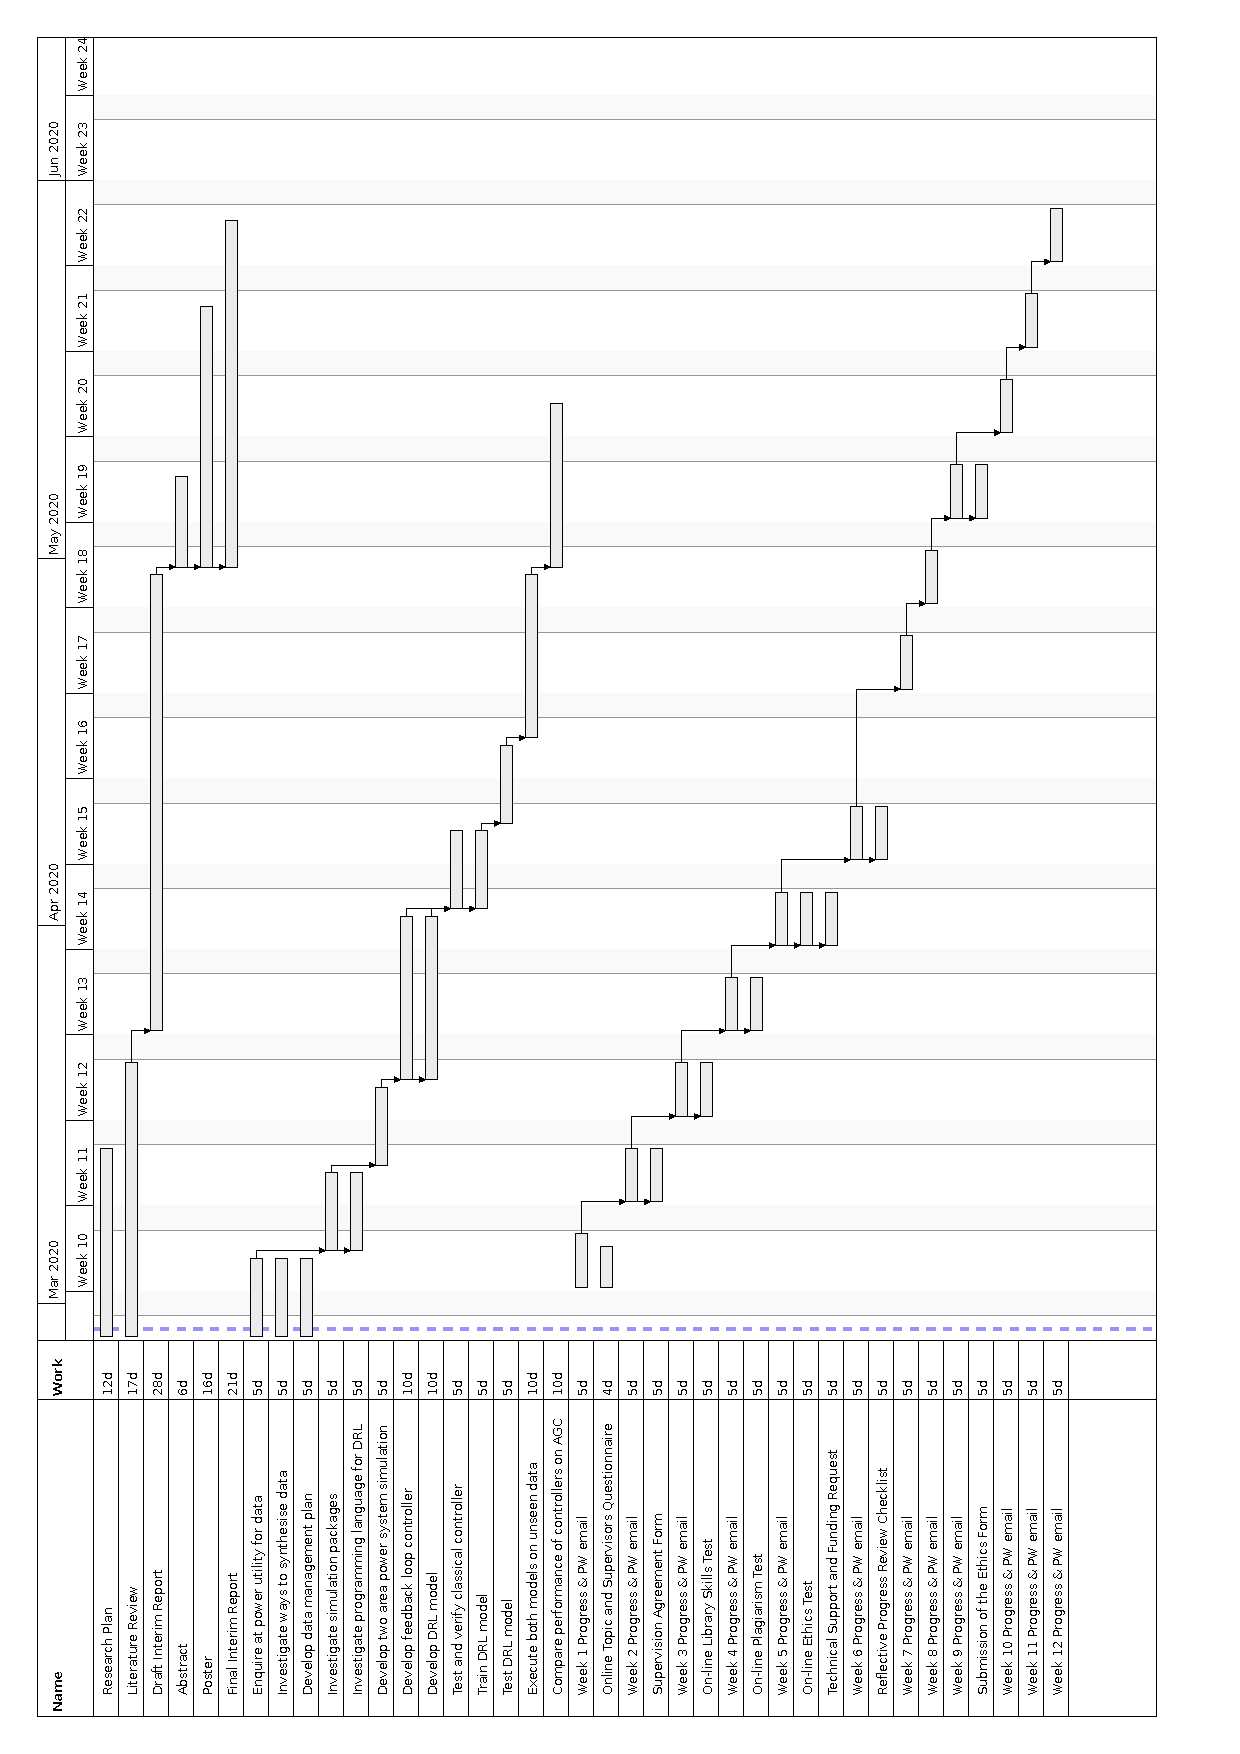
\includegraphics[scale=0.8]{./project_plan/project_plan}
	\caption{text}
\end{figure}

The timeline is not a static document; you will need to update it regularly.

\clearpage


%------------------------------------
% Expected Outcomes and Impacts
%------------------------------------
\section{Expected Outcomes and Impacts}
Conclude your research proposal by stating your expected outcomes. At this stage in the research process, what arguments and conclusions do you expect to reach? Your reader will understand that these are projected outcomes based on the extent of research at the time of writing, and that they will almost certainly change in the light of further research. It is essential, however, that you give your reader a sense of what conclusions may be drawn. This will allow your reader to further assess the significance and validity of your project. It will also indicate to your reader that you have thought ahead and considered the potential outcomes and implications of your research.

To avoid repetition with the description of your research aims and significance earlier in the proposal, focus on how you envisage your research will contribute to debates and trends in your field. What impact might your findings have on how the problem is perceived? What impact might your methods have on how research is conducted in the future?


%------------------------------------
%Bibliography
%------------------------------------
\bibliographystyle{unsrt}
\bibliography{./bib/my_bib}

\end{document}